\documentclass[conference]{IEEEtran}
\usepackage[T1]{fontenc}
\usepackage{cite,amsmath,amssymb,graphicx,booktabs,url}
\newcommand{\ugm}{\ensuremath{\mu\mathrm{g\,m}^{-3}}}
\title{Limits of Sub-THz VOC and Particulate Sensing with Communication-Pilot Reuse}
\author{\IEEEauthorblockN{Guillem Moreno Garcia}
\IEEEauthorblockA{Universitat Polit\`ecnica de Catalunya\\
Email: guillem.moreno.garcia@estudiantat.upc.edu}}
\begin{document}
\maketitle
\begin{abstract}
We evaluate whether communication pilots in a 60--400 GHz satellite downlink can support joint volatile-organic-compound (VOC) and particulate-matter (PM) estimation. An externally parameterized model combines isotope-resolved HITRAN spectroscopy, a refracted spherical atmosphere, microwave absorption and emission, Mie particle distributions, and explicit radio resources. Atmospheric radio observations remain simulated. For a 10 s ideal multiband reference with zero persistent residual and bias, conditional 95\%-power detection limits are 56.21, 131.24 and 12.94 micrograms per cubic metre for formaldehyde, methanol and acetonitrile. Fine/coarse PM information remains inadequate despite nonlinear fitting. A contiguous E-band OFDM control preserves communication resources under read-only pilot reuse but does not establish useful joint sensing. Independent public evidence adds a published 380 GHz humidity-response comparison and measured calcite-cell transmission in four native bins between 300 and 400 GHz. Reference drift and missing particle mass labels prevent a PM calibration claim. We distinguish completed numerical analyses, negative feasibility findings and missing experimental evidence. Neither instantaneous model sensitivity nor preserved modeled rate establishes environmental compliance or a validated atmospheric monitor.
\end{abstract}
\begin{IEEEkeywords}
Atmospheric sensing, volatile organic compounds, particulate matter, HITRAN, calibration, integrated sensing and communication.
\end{IEEEkeywords}

\section{Question and evidence}
Differential absorption has been studied for water vapour in sub-terahertz satellite contexts \cite{aliaga}; multi-medium propagation models also motivate joint gas and particle analysis \cite{yang}. We ask whether a specified satellite channel can distinguish weak VOC and PM signatures while preserving its communication resources.

Implementing a model, evaluating an estimator, and demonstrating an environmental monitor are different milestones. An evaluation may legitimately produce a negative feasibility result. A successful numerical optimizer or a small local error bound does not establish a calibrated measurement.

This revision supplies an expanded atmosphere and spectroscopy implementation, explicit detection probabilities, nonlinear-response checks, OFDM waveform and moving-pass controls, a PM information diagnosis, and bounded comparisons with public measured evidence. All sensing calculations remain in 60--400 GHz. The previous September 8 manuscript is preserved as a dated historical artifact.

\begin{table}[t]\centering\footnotesize
\caption{Evidence types and supported interpretations.}
\begin{tabular}{p{.27\columnwidth}p{.62\columnwidth}}\toprule
Evidence & Interpretation\\\midrule
HITRAN catalogue & External spectroscopy; not measured atmospheric CSI.\\
Beijing surface data & Measured scenarios; not vertical pollutant profiles.\\
IGRA soundings & Measured weather; upper continuation is modeled.\\
Simulated pilots & Conditional estimator and detector controls.\\
Published 380 GHz results & Independent aggregate water-background check.\\
Public calcite THz-TDS & Measured cell response/drift; no PM mass labels.\\\bottomrule
\end{tabular}\label{tab:evidence}
\end{table}

\section{Atmosphere, spectroscopy and particles}
\subsection{Weather and concentration profiles}
The reference atmosphere implements ITU-R P.835-7 Annex 1 through 100 km, including height conventions and atmospheric interfaces \cite{itu835}. NOAA IGRA data supply Beijing pressure, temperature, height and dew-point depression \cite{igra}. Parsing retains 103,322 levels from 521 soundings. A fixed rule selects the first complete profile reaching at least 20 km in January, April, July and September 2026. Measured tops range from 28.8 to 37.0 km above the station. Temperature and logarithmic pressure/vapour are interpolated; continuation above the measured top is explicitly modeled.

Weather soundings do not measure VOC or PM abundance profiles. Gas and dry-particle concentrations remain proportional to $\exp(-z/H)$ with declared scale heights of 1,500 and 1,000 m. The four weather profiles are examples, not a population distribution, and are not paired with the historical PM record or radio observations. Horizontal homogeneity and nondispersive ray refraction remain assumptions.

\subsection{Spectroscopy and refracted integration}
The acquired inventory contains 34 isotope tables, 304,416 catalogue transitions and 31,474 transitions in 60--400 GHz. Formaldehyde, methanol and acetonitrile are the VOC targets; CO, O$_3$, SO$_2$ and NO$_2$ are interfering gases. Methane is retained as an acquisition control. Out-of-band line centres contribute tails only. Three additional isotope/window requests were unavailable and remain failed requests, not zero absorption.

For molecule $s$, the local absorption cross-section is
\begin{equation}
\sigma_s(\nu,z)=\sum_{\ell\in s} S_\ell(T(z))
V_\ell[\nu-\nu_\ell-\delta_\ell p(z);T(z),p(z)],
\end{equation}
with temperature-dependent line strengths, partition sums, pressure shifts and air/self broadening \cite{hitran,hapi}. Voigt profiles combine pressure and Doppler effects. Each isotope uses its mass and partition sum; terrestrial abundance is not multiplied twice. Natural-mixture molar masses define reported mass/ppm conversions.

The attenuation is
\begin{equation}
A_s(\nu)=\frac{10}{\ln10}\int_{\mathrm{ray}}n_s(z)\sigma_s(\nu,z)\,ds.
\end{equation}
Bouguer's invariant $b=n(r)r\sin\zeta$ defines a spherical refracted path connecting the receiver and satellite. Quadrature respects atmospheric interfaces, replacing a secant multiplication of a completed vertical column.

P.676-13 Annex 1 supplies microwave oxygen/water absorption, line-mixing and continuum terms \cite{itu676}. It replaces HITRAN H$_2$O/O$_2$ in the current background, avoiding double counting. Twelve additional rare-isotope comparisons against HAPI pass with maximum peak-normalized discrepancy about $7.70\times10^{-6}$. HAPI shares the line data: this checks implementation, not independent physical truth. Missing broadening and parameter-uncertainty distributions limit unconditional claims. Far-wing truncation remains a sensitivity control.

\subsection{Particles, emission and numerical checks}
Full homogeneous-sphere Mie extinction is integrated over truncated lognormal number distributions and normalized by dry mass \cite{mie}. Fine/coarse modes use aerodynamic cuts and Stokes/Cunningham conversion; PM$_{10}$ is their sum. A supplied humidity-growth interface has an explicit effective-medium assumption. Target aerosol optical constants, composition, shape and humidity response remain uncalibrated.

Rayleigh-versus-Mie relative RMS differences are approximately 0.00086\% for fine particles and 0.0201\% for coarse particles. Agreement in this size/frequency regime does not add independent measurement information.

With $J_\nu(T)=(h\nu/k)/[\exp(h\nu/kT)-1]$, atmospheric thermal transfer gives
\begin{equation}
T_{\rm sky}=\sum_iJ_\nu(T_i)(1-e^{-\tau_i})e^{-\sum_{j<i}\tau_j}
+J_\nu(T_{\rm space})e^{-\sum_i\tau_i}.
\end{equation}
Receiver noise is $kB[T_{\rm sky}+T_0(F-1)]$; noise figure is not counted twice.

The numerical acceptance criterion is relative vector RMS difference below 0.1\% between two quadrature orders. The initial thermal comparison failed at 0.11596\%. Refining intervals to 100 m below 20 km and 500 m above reduced it to 0.00319\%, without changing the tolerance or other physics arrays. Gas, PM and background differences are 0.00381\%, 0.0225\% and 0.00200\%. An independent recursive transfer calculation reproduces the refined brightness. This establishes numerical stability on the tested grid, not atmospheric accuracy. The correction changes broad-reference rate by only about $-0.000270\%$.

The four measured-weather spectra use order two. Only the September profile has a separate order comparison, at 0.05304\% relative RMS; four independently converged weather runs are not claimed.

\section{Radio and inference model}
\subsection{Resources and pilot observations}
The reference link uses a 550 km satellite, $45^\circ$ elevation, 23 dBm total power, 0.50/0.30 m transmit/receive apertures, 6 dB noise figure and 5 dB implementation loss. The broad case has 256 separated frequencies in 60--400 GHz and is an ideal simultaneous multiband experiment.

The explicit E-band case has 256 contiguous 1 MHz tones centred at 73.5 GHz, one RF chain, a $1/16$ cyclic prefix and 30 pilots per 10,000-symbol frame. Its 73.372--73.628 GHz interval lies within the 71--76 GHz space-to-Earth reference discussed by ITU \cite{itu178}. This is not a coordination or licensing determination. WR12 laboratory VNA extenders cover this interval but are not flight-modem validation \cite{vdi}.

After reference normalization and assumed phase tracking, the complex pilot mean is
\begin{equation}
\bar z_i=10^{-[D\theta+N\beta]_i/20}+\eta_i,\qquad
\eta_i\sim\mathcal{CN}(0,(N_p\gamma_i)^{-1}),
\end{equation}
where $D$ holds three VOC and two PM signatures, and $N$ holds background/calibration and interfering-gas terms. Magnitude-derived attenuation is $-20\log_{10}|\bar z_i|$. Its local thermal variance is $2(10/\ln10)^2/(N_p\gamma_i)$. Separate scenarios add persistent correlated residuals. Covariance and SNR are conditional on the reference channel. The retained 5 dB single-pilot SNR mask is not a universal sensing threshold.

\subsection{Estimation, bias and detection}
For $y=D\theta+N\beta+n$, set $LL^T=\Sigma$, $\widetilde D=L^{-1}D$, and let $Q$ span $L^{-1}N$. With $P=I-QQ^T$, the efficient local estimator is
\begin{equation}
\widehat\theta=Hy,\quad H=(\widetilde D^TP\widetilde D)^{-1}\widetilde D^TP L^{-1}.
\end{equation}
Its covariance attains the nuisance-adjusted Gaussian bound when the target is identifiable \cite{kay}. SVD implementation and checks of retained column size prevent a removed signature from being normalized into false information.

The nonlinear diagnostic fits the exact complex mean, with Gaussian real/imaginary samples and concentrations bounded to 0--1,000 \ugm. It retains optimizer status, active bounds and profile likelihoods. Unknown phase tracking is not silently solved. Signed estimates, rather than clipped values, determine reported error and detection.

For persistent $\|b\|_\infty\le\epsilon$, the local worst-case concentration bias is $B_j=\epsilon\|h_j\|_1$. More pilots do not remove this term. Earlier Gaussian attainability work covers 48 configurations with 10,000 draws each and demonstrates strong sensitivity to persistent model mismatch; it remains archived.

Six reported targets include three VOCs, fine PM, coarse PM and PM$_{10}$. Bonferroni allocation uses family-wise false-positive budget $\alpha=0.01$ and required power 0.95. With standard error $s_j$,
\begin{align}
c_{\rm crit,j}&=z_{1-\alpha/6}s_j+B_j,\\
c_{\rm LOD,j}&=(z_{1-\alpha/6}+z_{0.95})s_j+2B_j.
\end{align}
The factor two covers opposite worst-case biases under null and alternative. Bonferroni permits dependent PM-derived targets. This rule is stricter than the previous 1\% per target and is unrelated to the numerical integration tolerance.

The grid attempts two bands, three nuisance policies, three durations (0.1, 10 and 1,800 s), and two residual levels: 36 configurations. Each evaluated case has 5,000 present and 5,000 absent controls. VOC injections are 1 \ugm; fine/coarse PM are 49/41 \ugm from one recorded Beijing scenario \cite{beijing}. These are response controls, not an environmental population. Precision assumes artificial 50\% prevalence. The retained tables have 114 detection, 228 error and 342 decision-limit rows; failed configurations are preserved.

\section{Conditional sensing results}
\subsection{VOCs and nuisance effects}
Table~\ref{tab:voc} uses the 10 s ideal broad reference, reference nuisance calibration, zero persistent residual and zero bias allowance. Recall at 1 \ugm\ is very low. At the larger predicted detection limits, new exact-response checks achieve 95.16\%, 95.40\% and 94.92\% recall, within the declared one-percentage-point tolerance of 95\%. These checks support three modeled operating points, not every uncertainty scenario or field performance.

\begin{table}[t]\centering\scriptsize
\caption{Broad 10 s reference. LOD assumes 95\% power and 1\% family-wise false positives. Recall and RMSE use 1 \ugm\ injections. ppm uses 288.15 K and 101325 Pa.}
\setlength{\tabcolsep}{3pt}
\begin{tabular}{lrrrr}\toprule
VOC & LOD (\ugm) & ppm & Recall (\%) & RMSE (\ugm)\\\midrule
Formaldehyde & 56.21 & 0.04426 & 0.30 & 12.44 \\
Methanol & 131.24 & 0.09685 & 0.20 & 28.71 \\
Acetonitrile & 12.94 & 0.00745 & 0.20 & 2.83 \\
\bottomrule\end{tabular}

\label{tab:voc}
\end{table}

Weather and smooth-instrument nuisance terms remove additional information. Seventeen of 18 E-band configurations fail the numerical audit. The remaining 1,800 s case has formal limits far beyond meaningful atmospheric interpretation and exceeds a single pass. Its marginal numerical rank does not establish useful sensing. The result rejects this evaluated design, not every possible E-band waveform.

\subsection{PM information and auxiliary requirements}
Formal local PM detection limits are about $4.85\times10^8$, $5.96\times10^8$ and $1.10\times10^8$ \ugm\ for fine, coarse and total PM. These are failure diagnostics, not validated concentration ranges. All 20 nonlinear fits report success, yet fine PM reaches a bound in 100\% and coarse PM in 95\%. The fine-PM likelihood is nearly flat across the fitted domain.

Projecting both PM columns against all gas/background nuisance terms gives correlation 0.999999962. Scenarios $(49,41)$ and approximately $(2.45,98.13)$ \ugm\ have optimized-nuisance separation only $4.39\times10^{-7}$ noise standard deviations. The conditional optimal equal-prior binary error is essentially 50\%.

Even fixing the other PM mode leaves standard errors of about 29,106 and 35,722 \ugm. Weak absolute sensitivity therefore remains after removing fine/coarse ambiguity. Hypothetical independent fine and total mass observations with 5 \ugm\ standard error reduce fine/coarse errors to approximately 5 and 7.07 \ugm. That information comes from the auxiliary observations, not THz retrieval.

\begin{figure*}[t]\centering
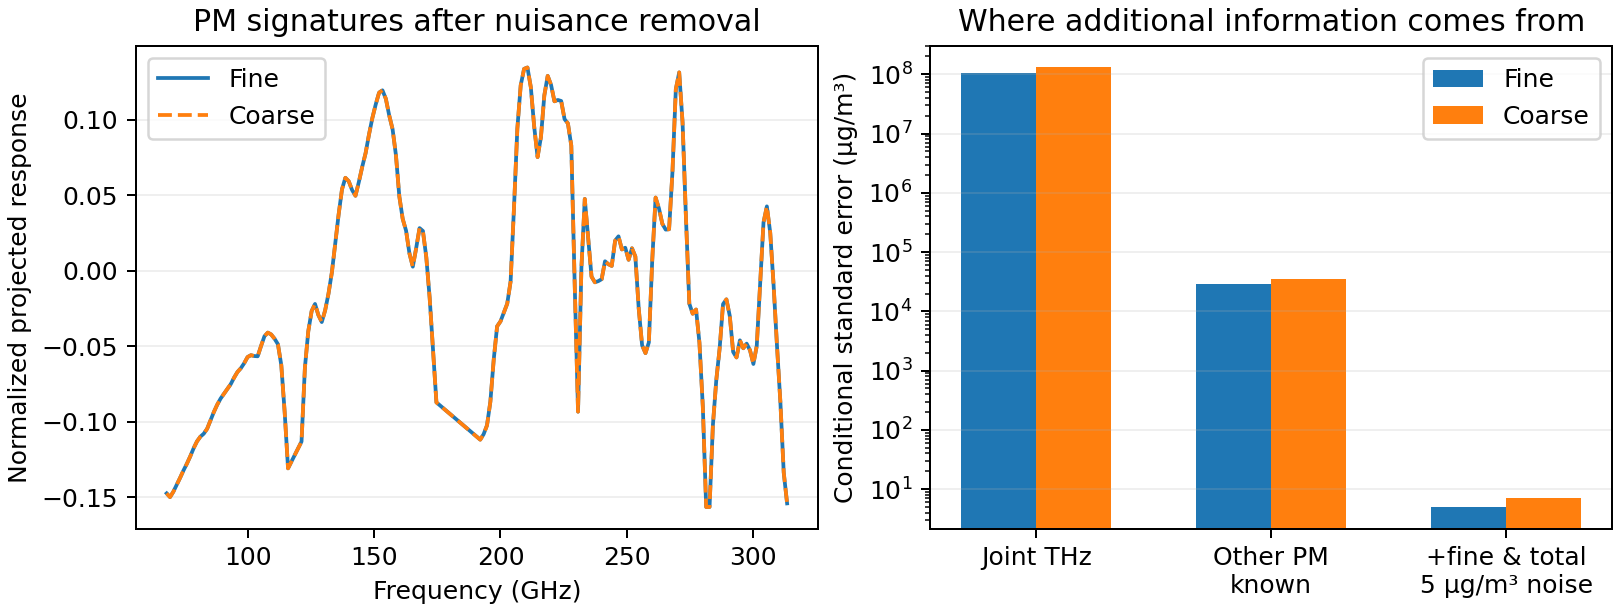
\includegraphics[width=.9\textwidth]{../results/five_task_closure/pm_information_diagnosis.png}
\caption{Projected PM responses and conditional uncertainty. The final bars require hypothetical calibrated mass observations; they are requirements analysis, not acquired data.}
\end{figure*}

\section{Communication and acquisition controls}
Communication-only and pilot-reuse sensing keep channel, power and required pilots identical. Modeled net information rates are 783.5117 Mbit/s for the broad reference and 763.4401 Mbit/s for E-band, with zero incremental reuse loss. Extra pilots, retuning or hardware are not assumed free.

A waveform control generates one 10,000-symbol OFDM frame, adds a cyclic prefix and complex time-domain noise, estimates the channel from 30 pilots and decodes uncoded QPSK. Each case scores 5,104,640 payload bits. Sensing reads a copy of the pilot CSI, leaving decoded bits unchanged. The uncoded payload rate is 480.44 Mbit/s, distinct from Shannon information rate. Table~\ref{tab:waveform} records residual CFO after ideal per-symbol common-phase tracking; no FEC or measured RF response is implied.

\begin{table}[t]\centering\footnotesize
\caption{OFDM controls with the same seed across impairment cases. Read-only sensing reuse preserves payload decisions.}
\begin{tabular}{rrrr}\toprule
CFO (kHz) & Bit errors & BER (\%) & Reuse decisions\\\midrule
0 & 12,700 & 0.2488 & Identical \\
10 & 12,891 & 0.2525 & Identical \\
100 & 34,540 & 0.6766 & Identical \\
\bottomrule\end{tabular}

\label{tab:waveform}
\end{table}

Seventeen snapshots of an ideal circular overhead pass recompute refracted background absorption, sky emission, range and instantaneous power allocation. Above $45^\circ$, the pass lasts 139.73 s and averages 912.99 Mbit/s in the model. Sampled carrier Doppler reaches 1.211 MHz. This reference excludes Earth rotation, weather availability, FEC and a demonstrated tracking loop.

Separate impairment calculations allow about 29.01 kHz residual CFO or 0.0526 rad RMS phase jitter for a 1\% information-rate loss. They are not a joint error budget. WR12 laboratory specifications quote typical 0.1 dB magnitude and $1.5^\circ$ phase stability after warm-up under stated conditions \cite{vdi}; these are not a stochastic covariance or receiver calibration recordings.

The E-band design is retained as a concrete communication reference and rejected as the current joint-sensing solution. A laboratory 260--400 GHz extender could examine the aerosol overlap, but a swept VNA scan is not simultaneous OFDM acquisition. A useful broad sensing system still needs feasible bands and measured tracking/calibration performance.

\begin{figure*}[t]\centering
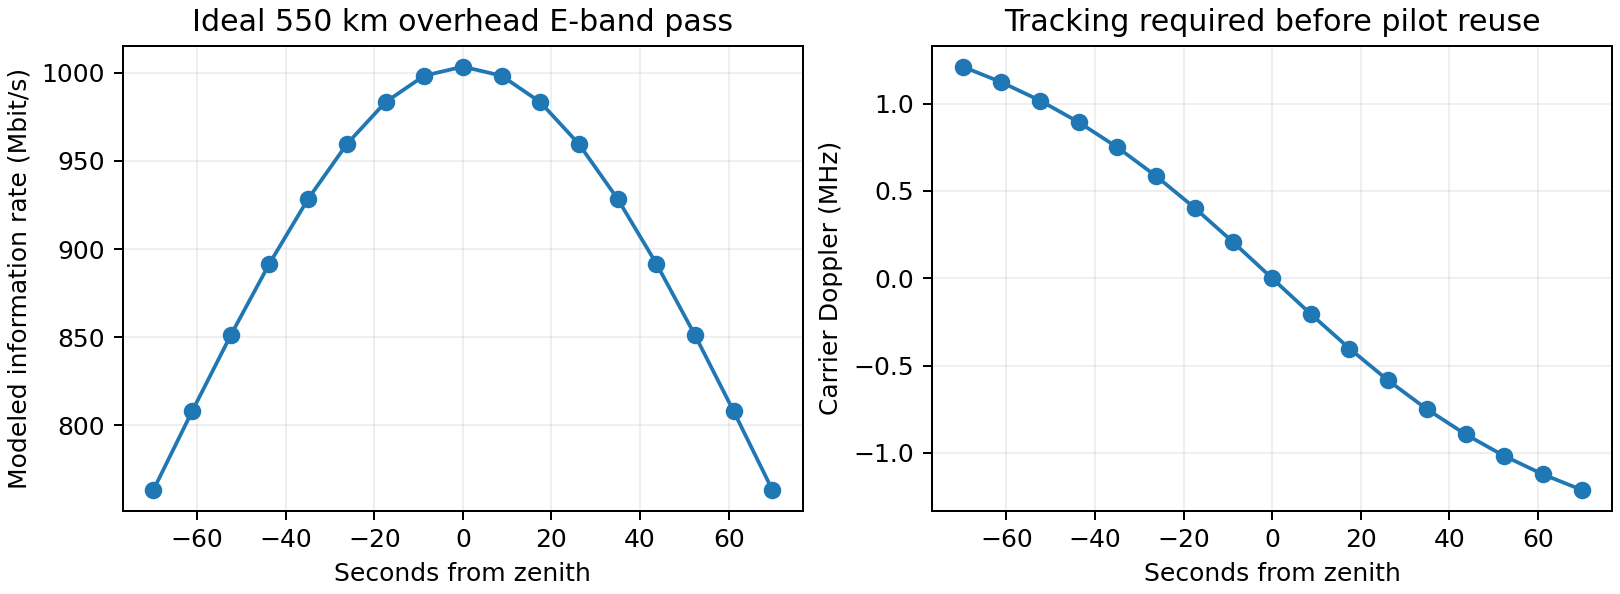
\includegraphics[width=.9\textwidth]{../results/five_task_closure/eband_moving_pass.png}
\caption{Ideal moving-pass reference. Same-channel sensing reuse preserves modeled resources; this does not demonstrate tracking, atmospheric availability or useful pollutant retrieval.}
\end{figure*}

\section{Independent public measurement checks}
\subsection{Water-background comparison}
Taleb et al. report atmospheric-pressure chamber measurements \cite{taleb}. Their Figure 8 gives 380 GHz humidity/attenuation slopes of $0.033\pm0.009$ for VNA and $0.027\pm0.009$ for THz-TDS in $(\mathrm{dB/m})/(\mathrm{g/m^3})$. We compare our implementation on a declared unsaturated humidity envelope at six temperatures and each instrument's reported pressure, without reconstructing their exact regression samples.

The VNA-pressure mean model slope is 0.0328; all six states fall within the reported VNA range. Some TDS-pressure states fall outside its reported range, and that discrepancy is retained. Raw measurements are author-request only. This is an aggregate independent water check, not VOC/PM or satellite validation; no confidence-level interpretation is imposed on the reported plus/minus values.

\begin{figure}[t]\centering
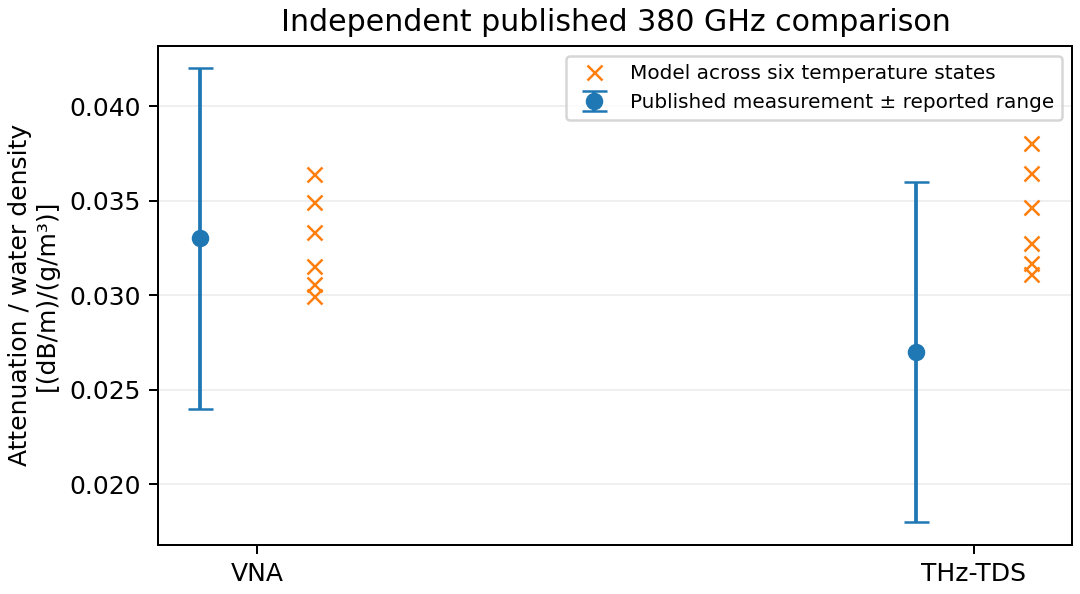
\includegraphics[width=\columnwidth]{../results/five_task_closure/published_water_validation.png}
\caption{Published water response and calculated state envelope at 380 GHz. Error bars reproduce reported ranges; crosses are our modeled states.}
\end{figure}

\subsection{Measured calcite aerosol controls}
Eliet's public dataset provides a one-metre dry-nitrogen calcite cell with corrected THz-TDS means and before/after blanks \cite{calcite}. Eight sample means and four blanks are reprocessed. Forty-picosecond traces yield approximately 25 GHz native resolution. The source declares useful signal above 300 GHz; only four native bins near 300, 325, 350 and 375 GHz remain within our frequency window. Zero padding is not used to manufacture resolution.

We calculate $-20\log_{10}|E_s/E_r|$ using geometric-mean blank amplitudes and log-amplitude interpolation between slightly different native grids. Before/after blank changes reach 0.090 dB, while repeat-blank differences stay below 0.01 dB. Across both blank choices, 42 of 64 apparent attenuation values are negative. They are retained as reference-sensitivity evidence, not clipped into particle absorption.

The inspected metadata contain no paired mass concentration or size distribution. Therefore these files cannot establish mass extinction or PM calibration. Calcite in dry nitrogen also differs from mixed ambient aerosol. The result is measured transmission/drift evidence within a limited overlap, not validated PM$_{2.5}$/PM$_{10}$ recovery.

\begin{figure*}[t]\centering
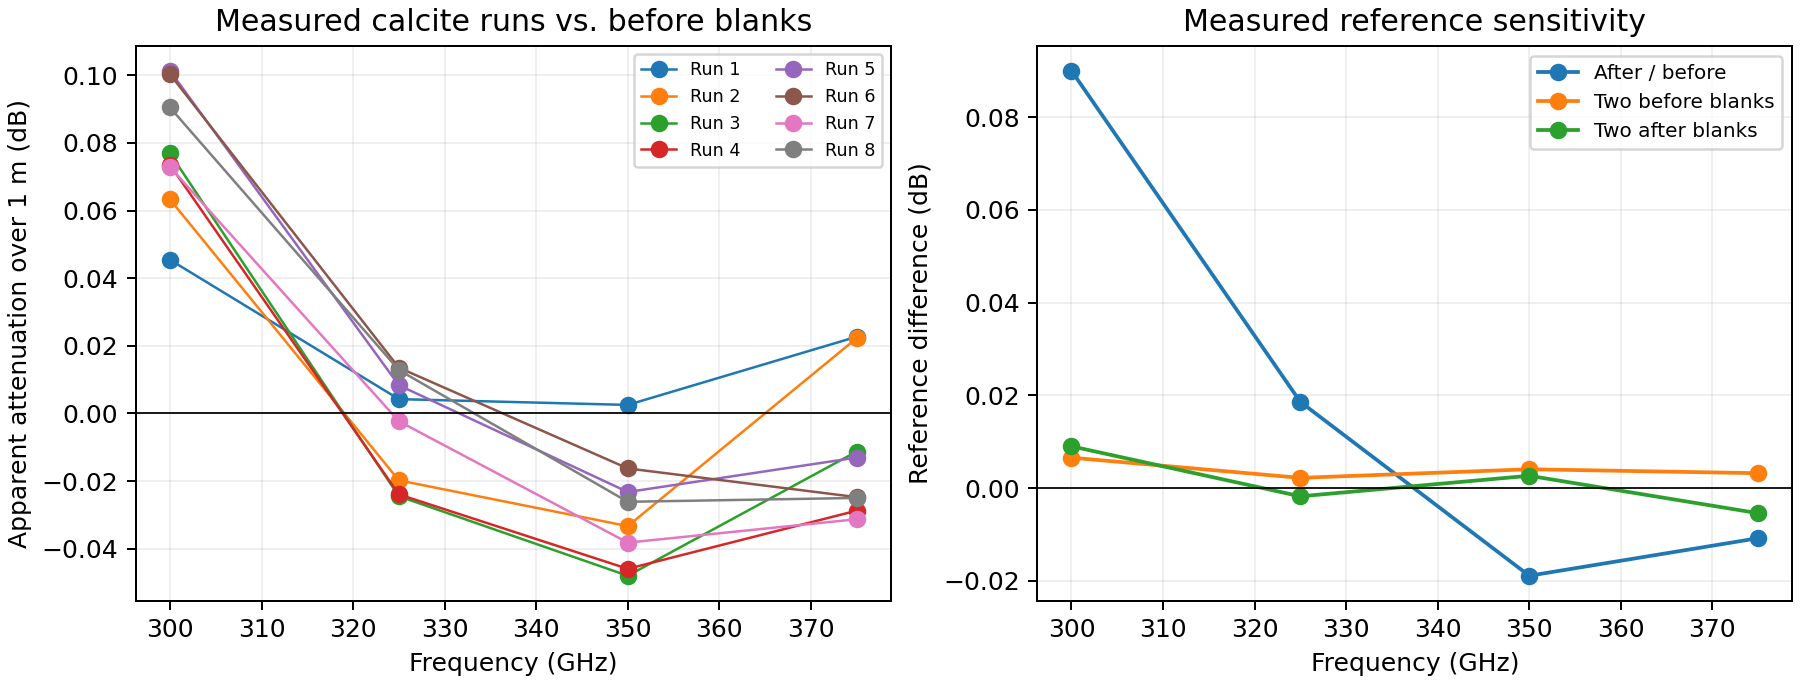
\includegraphics[width=.9\textwidth]{../results/five_task_closure/public_calcite_validation.png}
\caption{Measured calcite response and blank sensitivity in four native in-band bins. Lines are visual connections. No mass-concentration labels are available.}
\end{figure*}

\subsection{VOC evidence screened}
An in-band acetonitrile experiment around 165 GHz demonstrates laboratory rotational spectroscopy, but uses low-pressure cells, fitted pressure interpretation and long sequential scans \cite{gudz}. It cannot validate ambient satellite sensitivity. A located open methanol dataset operates around 3.4 THz and is excluded \cite{leeds}. No matched atmospheric VOC/PM radio validation dataset was acquired in this bounded search.

\section{Environmental requirements and completion boundary}
WHO concentration guidelines have specific measurement domains and averaging periods \cite{who2021,who2010}; they are not instrument-accuracy specifications. The assessment separates domain, temporal coverage, paired reference data, calibration and conditional sensitivity.

Ambient PM$_{2.5}$/PM$_{10}$ daily values are 15/45 \ugm, with annual values 5/15 \ugm. Daily assessment also requires its annual percentile context. The 10 s modeled PM limits exceed daily concentration scales by about $3.24\times10^7$ and $2.45\times10^6$. Even an unrealistically continuous independent-noise 24-hour extrapolation gives formal limits near $5.22\times10^6$ and $1.19\times10^6$ \ugm. These extreme values diagnose missing information, not valid extrapolated sensing ranges.

Formaldehyde's 100 \ugm\ reference is a 30-minute indoor guideline. The outdoor slant observation has the wrong domain despite a smaller modeled LOD. An ideal pass above $45^\circ$ covers only 7.76\% of 30 minutes and 0.162\% of a day. A stationary 1,800 s control is not continuous coverage or a constellation schedule. The selected WHO sources do not provide ambient methanol/acetonitrile limits; occupational limits are not substituted.

This completes an evidence-based negative/unverified requirements assessment, not compliance verification. Likewise, numerical implementations of atmosphere, spectra, slant integration, PM scattering, CSI, estimators, bounds and declared sensitivity studies do not establish field validation.

\begin{table}[t]\centering\footnotesize
\caption{Five requested closure areas.}
\begin{tabular}{p{.24\columnwidth}p{.65\columnwidth}}\toprule
Area & Outcome and remaining boundary\\\midrule
Environmental criteria & Domain/period/detection assessment done; compliance absent.\\
Practical radio & OFDM, pass and impairment controls done; E-band sensing rejected.\\
PM limitation & Information diagnosis and measured aerosol reanalysis done; mass calibration absent.\\
Physical validation & Aggregate water and measured aerosol checks done; paired VOC/PM transmission absent.\\
Deliverables & Updated manuscript, evidence, scripts and measurement protocol.\\\bottomrule
\end{tabular}
\end{table}

\section{Reproducibility and next experiment}
Completion arrays reside in \texttt{results/task\_completion}; new measurements, analyses and figures are in \texttt{results/five\_task\_closure}. Table rows are generated from saved CSV/JSON. Source hashes, direct dependency versions, build instructions, tests and numerical checks accompany the revision. Raw data are acquired by script and checked against repository checksums when supplied. Historical failures and manuscripts are preserved.

Software tests do not validate environmental assumptions. Published water agreement cannot determine the complete background covariance. Calcite-cell drift cannot be transplanted into a satellite receiver's noise law. Four soundings do not define population uncertainty. New diagnostics on previously studied data are not fresh confirmatory field trials.

The next experiment needs calibrated complex transmission; blanks before/after; independent gas concentrations and particle mass/size/composition; weather; timing; and traceable instrument calibration. Calibration and final evaluation campaigns must be separated before inspecting outcomes. The repository supplies a schema and frozen detection/averaging protocol without invented measurements. Those physical milestones remain open without suitable data and hardware.

\section{Conclusion}
The expanded study provides reproducible conditional limits and explicit negative design decisions. VOC operating points are internally testable, while low-concentration and joint PM performance remain inadequate. Existing-pilot sensing preserves modeled communication resources and waveform decisions, but the explicit E-band case does not combine that property with useful sensing. Public evidence strengthens particular background and calibration checks without closing atmospheric VOC/PM validation. The defensible outcome is a quantified feasibility boundary and measurement protocol, not a completed satellite pollution monitor.

\IEEEtriggeratref{10}
\begin{thebibliography}{18}
\bibitem{aliaga} S. Aliaga et al., ``Analysis of integrated differential absorption radar and subterahertz satellite communications beyond 6G,'' \emph{IEEE J. Sel. Topics Appl. Earth Obs. Remote Sens.}, vol. 17, pp. 19243--19259, 2024, doi: 10.1109/JSTARS.2024.3480816.
\bibitem{yang} Z. Yang, W. Gao and C. Han, ``A universal attenuation model of terahertz wave in space-air-ground channel medium,'' \emph{IEEE Open J. Commun. Soc.}, vol. 5, pp. 2333--2342, 2024, doi: 10.1109/OJCOMS.2024.3386759.
\bibitem{itu835} ITU-R, \emph{Reference standard atmospheres}, Recommendation P.835-7, 2024.
\bibitem{igra} NOAA NCEI, \emph{Integrated Global Radiosonde Archive}, version 2, Beijing 2026 station archive, accessed September 2026. \url{https://www.ncei.noaa.gov/products/weather-balloon/integrated-global-radiosonde-archive}
\bibitem{hitran} I. E. Gordon et al., ``The HITRAN2024 molecular spectroscopic database,'' \emph{J. Quant. Spectrosc. Radiat. Transf.}, 2026, doi: 10.1016/j.jqsrt.2026.109807.
\bibitem{hapi} R. V. Kochanov et al., ``HITRAN Application Programming Interface (HAPI): A comprehensive approach to working with spectroscopic data,'' \emph{J. Quant. Spectrosc. Radiat. Transf.}, vol. 177, pp. 15--30, 2016.
\bibitem{itu676} ITU-R, \emph{Attenuation by atmospheric gases and related effects}, Recommendation P.676-13, 2022, Annex 1.
\bibitem{mie} C. F. Bohren and D. R. Huffman, \emph{Absorption and Scattering of Light by Small Particles}. Wiley, 1983. Numerical implementation: miepython 3.0.2.
\bibitem{itu178} ITU-R, \emph{Allocation of ITU-R preparatory work for WRC-27}, Resolution 178 discussion, Circular Letter CA/251.
\bibitem{vdi} Virginia Diodes, \emph{VNA Frequency Extension Modules: Summary of Performance Specifications}, VDI-956, rev. March 17, 2022, accessed September 2026.
\bibitem{kay} S. M. Kay, \emph{Fundamentals of Statistical Signal Processing: Estimation Theory}. Prentice Hall, 1993.
\bibitem{beijing} S. Chen, ``Beijing Multi-Site Air Quality,'' UCI Machine Learning Repository, 2017, doi: 10.24432/C5RK5G.
\bibitem{taleb} F. Taleb et al., ``Propagation of THz radiation in air over a broad range of atmospheric temperature and humidity conditions,'' \emph{Scientific Reports}, vol. 13, art. 20782, 2023, doi: 10.1038/s41598-023-47586-8.
\bibitem{calcite} S. Eliet, ``TeraHertz time domain spectroscopy of calcite particles resuspended (aerosol form),'' Recherche Data Gouv, version 1, 2026, doi: 10.57745/DLJEFW. Acquired September 11, 2023; authors' corrected outputs use Correct@TDS.
\bibitem{gudz} D. Gudz et al., ``(Sub-)millimeter spectroscopy instrument for the soil metabolite detection,'' \emph{IEEE Sensors J.}, vol. 25, no. 22, pp. 41274--41281, 2025, doi: 10.1109/JSEN.2025.3614491.
\bibitem{leeds} M. D. Horbury et al., \emph{Data associated with Real-Time Terahertz Absorption Spectroscopy of Methanol and Deuterated-Methanol Vapour, using a TeraFET Detector Array}, University of Leeds, doi: 10.5518/1321. Screened and excluded from validation because it is out of band.
\bibitem{who2021} World Health Organization, \emph{WHO Global Air Quality Guidelines}, 2021, ISBN 9789240034228.
\bibitem{who2010} World Health Organization, \emph{WHO Guidelines for Indoor Air Quality: Selected Pollutants}, 2010, formaldehyde chapter, ISBN 9789289002134.
\end{thebibliography}
\end{document}
